\chapter{Numerische Ergebnisse}
\label{chap:numerische_ergebnisse}

In diesem Kapitel werden numerische Ergebnisse
der beiden Verfahren f�r verschiedene Testprobleme
vorgestellt.
Wir beschr�nken unseren Test auf
Optimierungsprobleme mit linearen Restriktionen.
Wir werden somit Optimierungsprobleme
mit nichtlinearen Restriktionen
wegen des h�hen Aufwands
nicht ber�cksichtigen.

%\section{Testfunktionen}
%Wir betrachten hier einige Testfunktionen, die als Zielfunktion
verschiedener restringierter Optimierungsaufgaben benutzt werden k�nnen.

\begin{testfunction}
Quadratische Funktion in $\R^n$
\[
  f(x) := \| x - d \|^2 = \sum_{k=1}^{n} (x_k - d_k)^2
\]
\end{testfunction}
Die erste Testfunktion ist eine einfache mehrdimensionale Parabel
mit Minimalstelle im Punkt~$d$ und Optimalwert~0.

\begin{testfunction}
Exponentielle Funktion
\[
  f(x) := e^{\|x\|^2} = e^{\sum_{k=1}^{n} x_k^2}
\]
\end{testfunction}
\begin{figure}[ht]
  \centering
  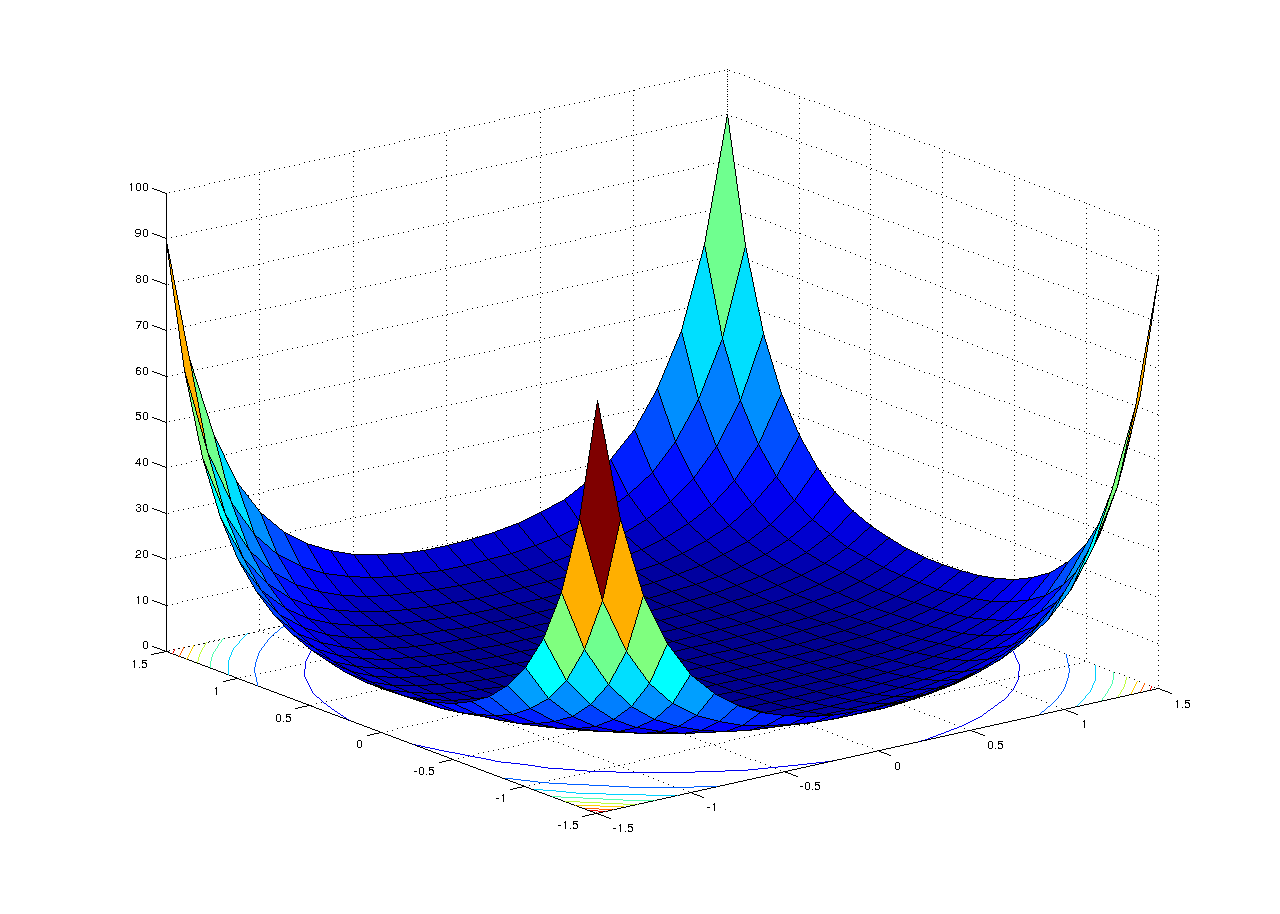
\includegraphics[width=0.75\textwidth]{exp-func}
  \caption{Exponentielle Funktion}
  \label{fig:exp_func}
\end{figure}
Die zweite Testfunktion ist eine exponentielle Funktion
mit Minimalstelle im Ursprung und Optimalwert~1.
Diese Funktion ist herausfordend, weil ihre Funktionswerte sehr schnell
gro� werden k�nnen.

\begin{testfunction}
Rosenbrock-Funktion
\[
  f(x) := 100(x_2-x_1^2)^2+(1-x_1)^2
\]
\end{testfunction}
\begin{figure}[ht]
  \centering
  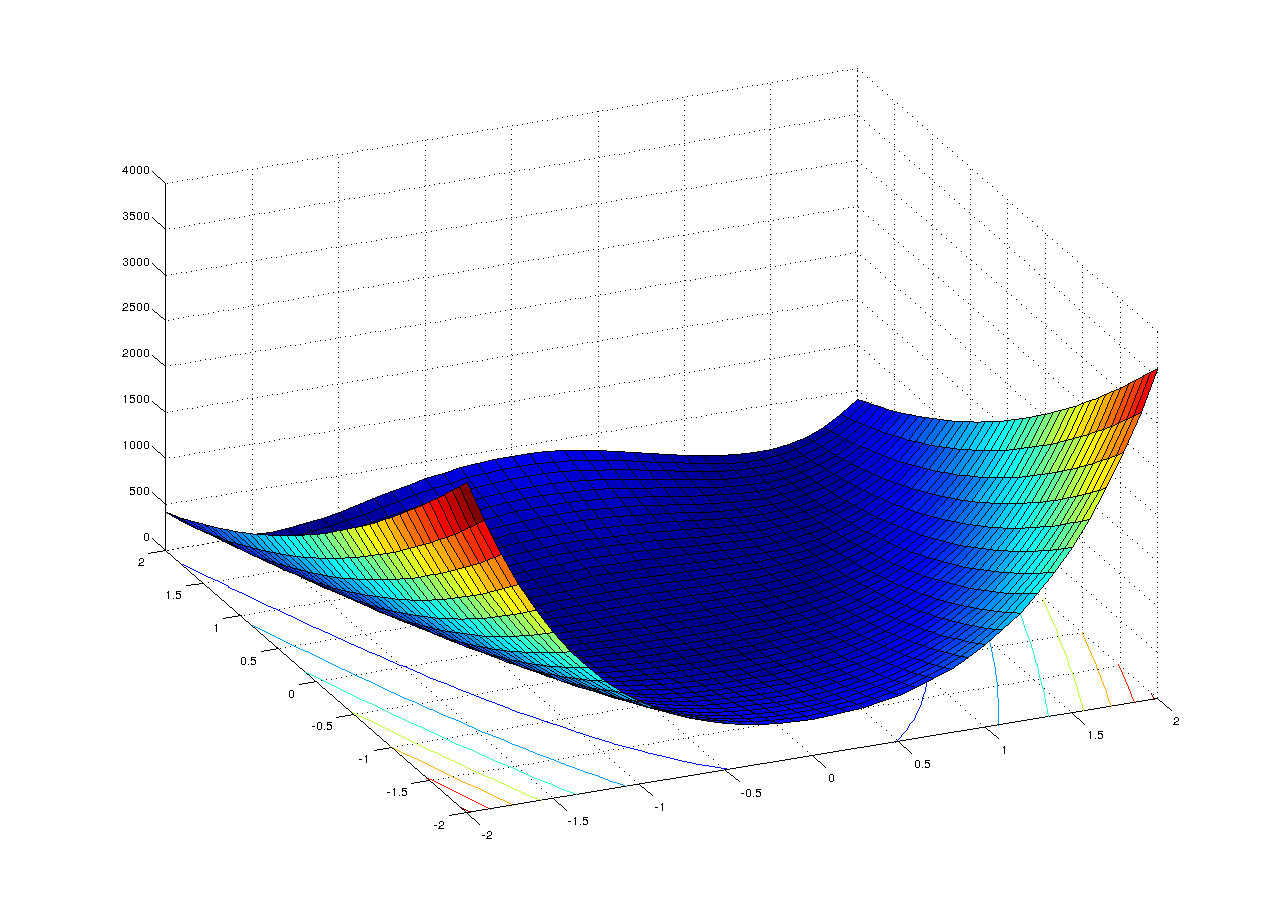
\includegraphics[width=0.75\textwidth]{rosenbrock}
  \caption{Rosenbrock-Funktion}
  \label{fig:rosenbrock}
\end{figure}
Die Rosenbrock-Funktion hat ein einziges Minimum
an der Stelle $\xopt = (1,1)^T$ mit $f(\xopt) = 0$.
Diese Funktion ist nicht einfach zu l�sen, da
das Minimum in einem schmalen "`bananenf�rmig"' gekr�mmten Tal liegt.
Als Anfangspunkt wird normalerweise den Punkt $x^0 = (-1,1)^T$ genommen.

\begin{testfunction}
Himmelblau-Funktion
\[
(x_1^2+x_2-11)^2 + (x_1+x_2^2-7)^2
\]
\end{testfunction}
\begin{figure}[ht]
  \centering
  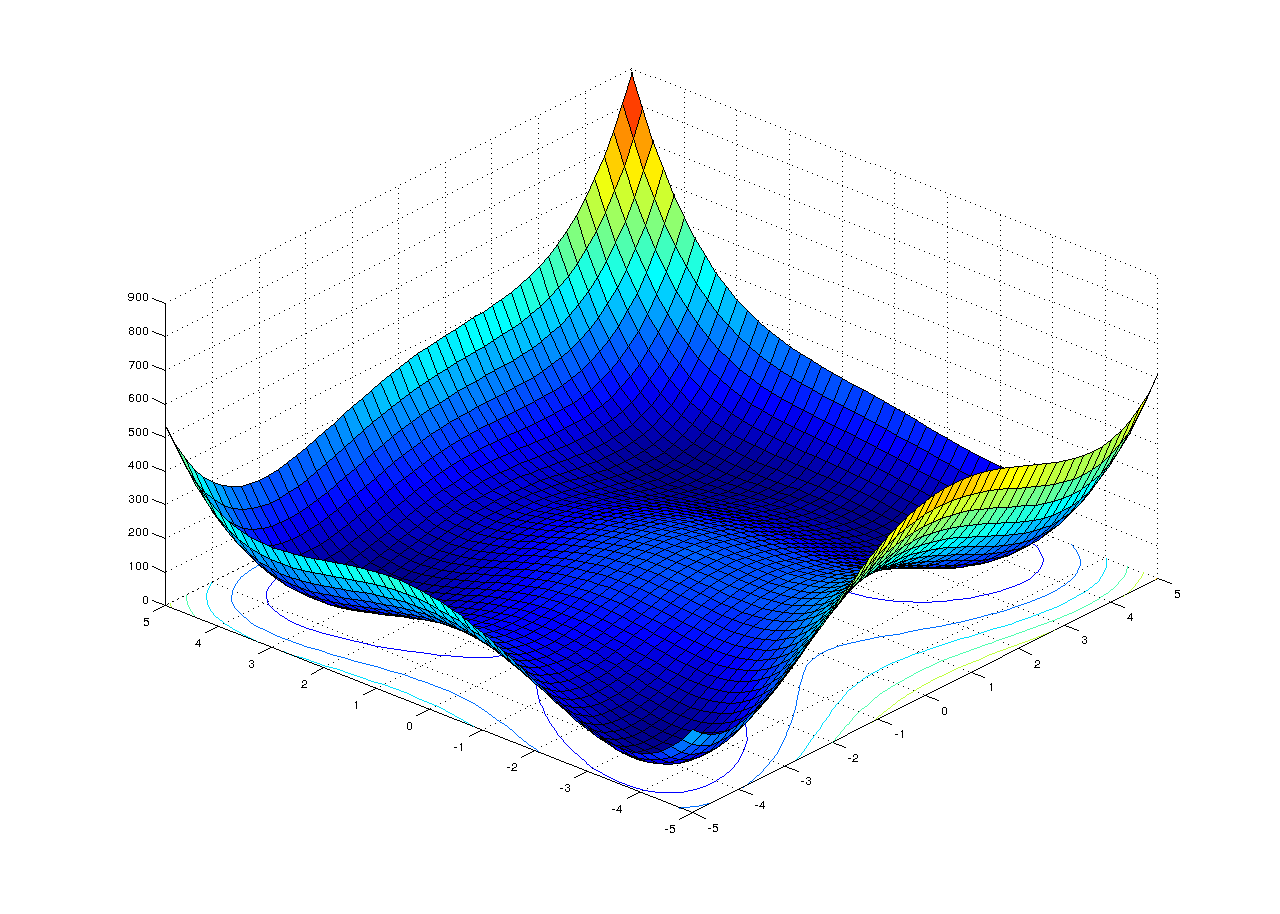
\includegraphics[width=0.75\textwidth]{himmelblau}
  \caption{Himmelblau-Funktion}
  \label{fig:himmelblau}
\end{figure}
Die Himmelblau-Funktion ist ein Polynom 4.~Grades
mit vier globale Minimalstellen.
Der Optimalwert ist 0.

\begin{testfunction}
Bazaraa-Shetty-Funktion
\[
  f(x) := (x_1-2)^4+(x_1-2x_2)^2
\]
\end{testfunction}
\begin{figure}[ht]
  \centering
  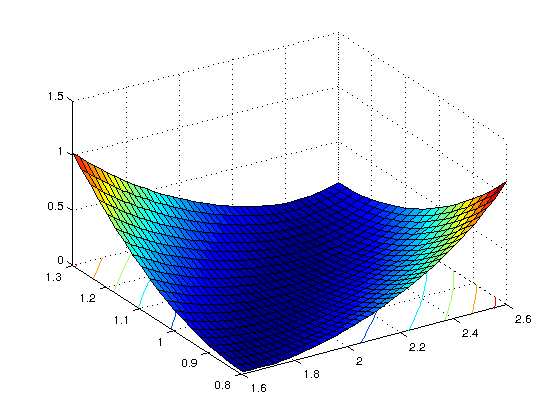
\includegraphics[width=0.75\textwidth]{bazaraa-shetty}
  \caption{Bazaraa-Shetty-Funktion}
  \label{fig:bazaraa_shetty}
\end{figure}
Die Bazaraa-Shetty Funktion ist ein Polynom 4.~Grades
mit einem globalen Minimum in $\xopt = (2,1)^T$
und Optimalwert 0.

\begin{testfunction}
Schuldt Funktion
\[
x_2+10^{-5}(x_2-x_1^2)^2
\]
\end{testfunction}

\begin{testfunction}
Asaadi Funktion
\[
x_2+\frac{1}{3}(x_1+1)^3
\]
\end{testfunction}

\begin{testfunction}
McCormick Funktion
\[
\sin(x_1+x_2) + (x_1-x_2)^2 - 1.5x_1 + 2.5x_2 + 1
\]
\end{testfunction}

\begin{testfunction}
Dixon Funktion
\[
(1-x_1)^2 + \sum_{k=1}^{9} (x_k^2-x_{k+1})^2 + (1-x_{10})^2
\]
\end{testfunction}

\begin{testfunction}
Colville Funktion
\begin{multline}
  f(x) := 100(x_2-x_1^2)^2 + (1-x_1)^2 + 90(x_4-x_3^2)^2 + (1-x_3)^2 \\
    + 10.1((x_2-1)^2 + (x_4-1)^2) + 19.8(x_2-1)(x_4-1) \notag
\end{multline}
\end{testfunction}

\begin{testfunction}
Betts Funktion
\[
2 - \frac{1}{2}x_1x_2
\]
\end{testfunction}

\begin{testfunction}
Paviani Funktion
\[
  f(x) := - (\ln(x_1-2))^2 - (\ln(10-x_1))^2
            - (\ln(x_2-2))^2 - (\ln(10-x_2))^2
\]
\end{testfunction}


\section{Testprobleme}

Die Testprobleme k�nnen in drei Gruppen geteilt werden.
Die erste Gruppe besteht aus Problemen nur
mit oberen und unteren Schranken.
Zu der zweiten Gruppe geh�ren die Probleme
mit linearen Gleichungsnebenbedingungen.
Die Probleme mit linearen Ungleichungsnebenbedingungen
kommen anschlie�end in die letzte Gruppe.

\begin{testproblem}
(vgl. Beispiel 16.2 in \cite[S.~452]{nocedal}
\begin{equation}
\min_{x\in\R^3}\ \tfrac{1}{2} x^T Q x + q^T x + c
\end{equation}
\begin{equation*}
\begin{split}
\nb x_1 + x_3 & = 3 \\
x_2 + x_3 & = 0 \\
\end{split}
\end{equation*}
\end{testproblem}

\begin{testproblem}
\begin{equation}
\min_{x\in\R^5}\ \| x-x_d \|^2
\end{equation}
\begin{equation*}
\begin{split}
\nb x_1 + x_2 + x_3 + x_4 + x_5 & = 1 \\
\end{split}
\end{equation*}
\end{testproblem}

\begin{testproblem}
(vgl. Problem 28 in \cite[S.~51]{hock})
\begin{equation}
\min_{x\in\R^3}\ \tfrac{1}{2} x^T Q x + q^T x + c
\end{equation}
\begin{equation*}
\begin{split}
\nb x_1 + 2 x_2 + 3 x_3 & = 1 \\
\end{split}
\end{equation*}
\end{testproblem}

\begin{testproblem}
(vgl. Problem 48 in \cite[S.~71]{hock})
\begin{equation}
\min_{x\in\R^5}\ \tfrac{1}{2} x^T Q x + q^T x + c
\end{equation}
\begin{equation*}
\begin{split}
\nb x_1 + x_2 + x_3 + x_4 + x_5 & = 5 \\
x_3 - 2 x_4 - 2 x_5 & = -3 \\
\end{split}
\end{equation*}
\end{testproblem}

\begin{testproblem}
(vgl. Problem 51 in \cite[S.~74]{hock})
\begin{equation}
\min_{x\in\R^5}\ \tfrac{1}{2} x^T Q x + q^T x + c
\end{equation}
\begin{equation*}
\begin{split}
\nb x_1 + 3 x_2 & = 4 \\
x_3 + x_4 - 2 x_5 & = 0 \\
x_2 - x_5 & = 0 \\
\end{split}
\end{equation*}
\end{testproblem}

\begin{testproblem}
(vgl. Problem 52 in \cite[S.~75]{hock})
\begin{equation}
\min_{x\in\R^5}\ \tfrac{1}{2} x^T Q x + q^T x + c
\end{equation}
\begin{equation*}
\begin{split}
\nb x_1 + 3 x_2 & = 0 \\
x_3 + x_4 - 2 x_5 & = 0 \\
x_2 - x_5 & = 0 \\
\end{split}
\end{equation*}
\end{testproblem}

\begin{testproblem}
(vgl. Problem 53 in \cite[S.~76]{hock})
\begin{equation}
\min_{x\in\R^5}\ \tfrac{1}{2} x^T Q x + q^T x + c
\end{equation}
\begin{equation*}
\begin{split}
\nb x_1 + 3 x_2 & = 0 \\
x_3 + x_4 - 2 x_5 & = 0 \\
x_2 - x_5 & = 0 \\
-10 \leq x_i & \leq 10,\ i = 1,\ldots,5 \\
\end{split}
\end{equation*}
\end{testproblem}

\begin{testproblem}
(vgl. Problem 49 in \cite[S.~72]{hock})
\begin{equation}
\min_{x\in\R^5}\ (x_1-x_2)^2 + (x_3-1)^2 + (x_4-1)^2 + (x_5-1)^6 
\end{equation}
\begin{equation*}
\begin{split}
\nb x_1 + x_2 + x_3 + 4 x_4 & = 7 \\
x_3 + 5 x_5 & = 6 \\
\end{split}
\end{equation*}
\end{testproblem}

\begin{testproblem}
(vgl. Problem 50 in \cite[S.~73]{hock})
\begin{equation}
\min_{x\in\R^5}\ (x_1-x_2)^2 + (x_2-x_3)^2 + (x_3-x_4)^4 + (x_4-x_5)^2 
\end{equation}
\begin{equation*}
\begin{split}
\nb x_1 + 2 x_2 + 3 x_3 & = 6 \\
x_2 + 2 x_3 + 3 x_4 & = 6 \\
x_3 + 2 x_4 + 3 x_5 & = 6 \\
\end{split}
\end{equation*}
\end{testproblem}

\begin{testproblem}
\begin{equation}
\min_{x\in\R^2}\ \tfrac{1}{2} x^T Q x + q^T x + c
\end{equation}
\begin{equation*}
\begin{split}
\nb 2 x_1 + x_2 & \leq 2 \\
x_1 - x_2 & \leq 1 \\
-x_1 - x_2 & \leq 1 \\
-2 x_1 + x_2 & \leq 2 \\
\end{split}
\end{equation*}
\end{testproblem}

\begin{testproblem}
(vgl. Beispiel 16.4 in \cite[S.~475]{nocedal})
\begin{equation}
\min_{x\in\R^2}\ \| x-x_d \|^2
\end{equation}
\begin{equation*}
\begin{split}
\nb -x_1 + 2 x_2 & \leq 2 \\
x_1 + 2 x_2 & \leq 6 \\
x_1 - 2 x_2 & \leq 2 \\
0 & \leq x_i,\ i = 1,2 \\
\end{split}
\end{equation*}
\end{testproblem}

\begin{testproblem}
(vgl. Beispiel 13.2 in \cite[S.~415f]{antoniou})
\begin{equation}
\min_{x\in\R^4}\ \tfrac{1}{2} x^T Q x + q^T x + c
\end{equation}
\begin{equation*}
\begin{split}
\nb -x_1 & \leq 0 \\
-x_2 & \leq 0 \\
x_1 + 2 x_2 & \leq 2 \\
-x_4 & \leq -2 \\
-x_3 - x_4 & \leq -3 \\
x_3 + 2 x_4 & \leq 6 \\
\end{split}
\end{equation*}
\end{testproblem}

\begin{testproblem}
(vgl. Problem 21 in \cite[S.~44]{hock})
\begin{equation}
\min_{x\in\R^2}\ \tfrac{1}{2} x^T Q x + q^T x + c
\end{equation}
\begin{equation*}
\begin{split}
\nb -10 x_1 + x_2 & \leq -10 \\
2 \leq x_1 & \leq 50 \\
-50 \leq x_2 & \leq 50 \\
\end{split}
\end{equation*}
\end{testproblem}

\begin{testproblem}
(vgl. Problem 35 in \cite[S.~58]{hock})
\begin{equation}
\min_{x\in\R^3}\ \tfrac{1}{2} x^T Q x + q^T x + c
\end{equation}
\begin{equation*}
\begin{split}
\nb x_1 + x_2 + 2 x_3 & \leq 3 \\
0 & \leq x_i,\ i = 1,2,3 \\
\end{split}
\end{equation*}
\end{testproblem}

\begin{testproblem}
(vgl. Problem 76 in \cite[S.~96]{hock})
\begin{equation}
\min_{x\in\R^4}\ \tfrac{1}{2} x^T Q x + q^T x + c
\end{equation}
\begin{equation*}
\begin{split}
\nb x_1 + 2 x_2 + x_3 + x_4 & \leq 5 \\
3 x_1 + x_2 + 2 x_3 - x_4 & \leq 4 \\
-x_2 - 4 x_3 & \leq -1.5 \\
0 & \leq x_i,\ i = 1,\ldots,4 \\
\end{split}
\end{equation*}
\end{testproblem}




\begin{testproblem}
L�se folgendes, einfaches, 2-dimensionales Problem.
\begin{align}
  \min_{x \in \R^2}\ (x_1 - 1)^2 + (x_2 &- 2.5)^2 \\
  \nb -x_1 + 2x_2 & \leq 2 \\
       x_1 + 2x_2 & \leq 6 \\
       x_1 - 2x_2 & \leq 6 \\
                0 & \leq x_1, x_2
\end{align}
\end{testproblem}

\begin{figure}[ht]
\centering
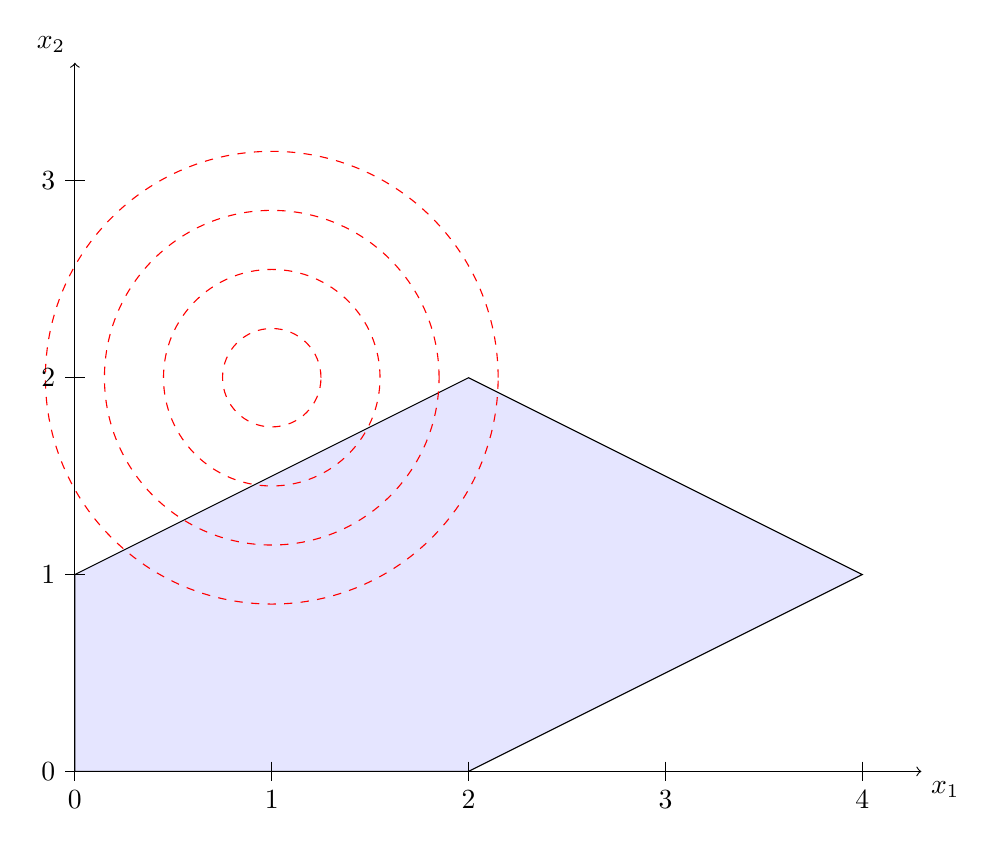
\begin{tikzpicture}[scale=2.5]
  
  % Die zul�ssige Menge
  \draw[fill=blue!10] (0,0) -- (0,1) -- (2,2) -- (4,1) -- (2,0) -- cycle;
  \draw (1.7,1) node {$\F$};
  
  % Die Niveaulinien
  \foreach \r in {0.25, 0.55, 0.85, 1.15}
    \draw[dashed,color=red] (1,2) circle (\r);
  
  % Koordinatenachsen
  \draw[->] (0,0) -- (4.3,0) node [below right] {$x_1$};
  \foreach \x in {0,...,4}
    \draw (\x,0.05) -- (\x,-0.05) node [below] {\x};
  \draw[->] (0,0) -- (0,3.6) node [above left] {$x_2$};
  \foreach \y in {0,...,3}
    \draw (0.05,\y) -- (-0.05,\y) node [left] {\y};
  
\end{tikzpicture}
\caption{Restringiertes Problem}
\end{figure}


